\section{Consistency study}
\label{sec:ND_Consistency}
In this section, we investigate the consistency of the
discretisation depending on the strategy used to treat the
surface layer. In particular, a special attention is paid to
the effect of changing $\delta_{\rm a}$.
Let $\delta_1$,$\delta_2$ two
different heights of surface layer
such that $\delta_1 < \delta_2$;
let $u_1$, $u_2$ be solutions of 
\eqref{eq:ND_NeutralCase_continuousModel} using
respectively $\delta_1, \delta_2$ for $\delta_{\rm a}$.
The main direct changes between $u_1$ and $u_2$ are:
\begin{itemize}
\item the Coriolis effect and the large-scale forcing are
taken into account in $[\delta_{1}, \delta_{2}]$
		only by $u_1$;
\item the viscosity $K_u(z)$ for $z \in [\delta_{1}, \delta_{2}]$
	is forced by the wall law to compute $u_2$
		and not to compute $u_1$.
\end{itemize}
There are also indirect effects due to the non-linearity of the
problem:
\begin{itemize}
	\item If the bulk algorithm is well designed it does not
		need the very top of the surface layer. Any height
		$z<\delta_{\rm a}$ within the wall law can be used
		to obtain the friction scales $u_\star$,
		$\theta_\star$: changing $\delta_{\rm a}$ does
		not \textit{directly} change the friction scales.
		However, the changes between $u_1$ and $u_2$ mentioned
		above indirectly change the output of the
		bulk algorithm.
		The friction scales $u_{\star, 1}$ and $u_{\star, 2}$
		are hence different.
\end{itemize}
\subsection{Study of the consistency: neutral case}
Figure \ref{fig:ND_Consistency_sensitivity_delta_sl} shows
three vertical profiles of $u$ obtained with
$\delta_{\rm a} = 5, 10$ and $20 \; {\rm m}$.
As expected, the angle Arg$(u)$
is constant in the surface layer because
the Coriolis effect is not taken into
account: changing $\delta_{\rm a}$
has an effect on the orientation of the wind.
Moreover, the vertical profile of $||u||$ above the
surface layer does not follow the wall law.
Consequently, the profile of $||u||$ depends strongly
on the choice of $\delta_{\rm a}$.
%
\begin{figure}
	\centering
\includegraphics[scale=0.6]{images/sensitivity_delta_sl.pdf}
	\caption{Typical profiles of $||u||$ and Arg$(u)$ for several
	choices of $\delta_{\rm a}$, obtained with the ``FV free"
	discretisation. Notice the changes of horizontal
	and vertical scales between the bottom and top panels.}
	\label{fig:ND_Consistency_sensitivity_delta_sl}
\end{figure}
\subsubsection{Analytical study of the sensitivity to $\delta_{\rm a}$}
\label{sec:ND_Consistency_sensitivity_delta_sl}
In this subsection we study the sensitivity to $\delta_{\rm a}$
of the continuous solution of
\eqref{eq:ND_NeutralCase_continuousModel}.
We will assume that the viscosity $K_u$ and the roughness length
$z_u$ are the same for both $u_1$ and $u_2$.
\par
In Figure \ref{fig:ND_Consistency_sensitivity_delta_sl} the value
of $z_u$ for $\delta_{\rm a} = 5\;{\rm m},10\;{\rm m},20\;{\rm m}$
is respectively $z_u = 3.8 \times 10^{-5} \;{\rm m},
3.8 \times 10^{-5} \;{\rm m}$ and $3.6 \times 10^{-5} \;{\rm m}$.
It seems reasonable to assume that $z_u$ do not depend on
$\delta_{\rm a}$ for this analytical study of the sensitivity to
$\delta_{\rm a}$.
\par
First, note that inside the surface layer for $u_2$,
since $u_2(z) = \frac{u_\star}{\kappa}\ln(1+\frac{z}{z_u})
\frac{u_2(\delta_{2})}{||u_2(\delta_{2})||}$, assuming
$||u_2(z)||$ follows the same wall low (it only works
when the problem is continuous in time), we have:
\begin{equation}
	(\partial_t + if) u_2(z) = \frac{\ln(1+\frac{\emphase{z}}{z_u})}
	{\ln(1+\frac{\emphase{\delta_2}}{z_u})}(\partial_t + if) u_2(\delta_2), 
~~~\forall z \leq \delta_2
\end{equation}
Let us assume that $K\partial_z u_2$ is
continuously differentiable at $\delta_2$;
then $\partial_z (K\partial_z u_2) = 0$ in all the interval
$(0, \delta_2)$ and the evolution equation of $u_2$ in
$(\delta_1, \delta_2)$ is
\begin{equation}
(\partial_t + if) u_2(z) = \frac{\ln(1+\frac{z}{z_u})}
	{\ln(1+\frac{\delta_2}{z_u})} \emphase{i f u_G}, 
	~~~\forall z \in (\delta_1, \delta_2)
\end{equation}
The difference between $u_1$ and $u_2$ is governed by
the difference of treatment of this interval:
subtracting the two evolution equations gives
\begin{equation}
	(\partial_t + if) (\emphase{u_2 - u_1}) =
	\emphase{\left(\frac{\ln(1+\frac{z}{z_u})}
	{\ln(1+\frac{\delta_2}{z_u})} - 1\right)i f u_G} 
-
\partial_z (K \partial_z u_1), ~~~\forall z \in (\delta_1, \delta_2)
\end{equation}
We see in the right hand side of the latter equation the two items
of the beginning of the section:
the large-scale forcing with the Coriolis effect,
and the diffusion term of $u_1$ which is actually
$\partial_z (K \partial_z u_1) = \partial_z (K \partial_z u_1 - K \partial_z u_2)$

Let $w=u_2 - u_1$. If we assume that $K$ is the viscosity for both
$u_2$ and $u_1$ then
\begin{equation}
	\begin{cases}
		(\partial_t + if) w = \partial_z (K \partial_z w) ,
		~~ \forall z > \delta_2 \\
(\partial_t + if) w = \partial_z (K \partial_z w)
		+ \emphase{\left(\frac{\ln(1+\frac{z}{z_u})}
		{\ln(1+\frac{\delta_2}{z_u})} - 1\right)i f u_G}
, ~~~\forall z \in (\delta_1, \delta_2) \\
		K \partial_z w = \frac{\kappa}
		{\ln(1+\frac{\delta_1}{z_u})}\left(
		u_{\star, 2} u_2(\delta_1) -
		u_{\star, 1} u_1(\delta_1)\right),
		~~~ \forall z \leq \delta_1
	\end{cases}
\end{equation}
Apart from the bulk sensitivity in the surface condition,
the difference comes hence from the forcing
$\left(\frac{\ln(1+\frac{z}{z_u})}
{\ln(1+\frac{\delta_2}{z_u})} - 1\right)i f u_G$.
This forcing is more important when $\frac{\delta}{z_u}$
is small. As it can be seen on Figure
\ref{fig:ND_Consistency_sensitivity_delta_sl}
the effect of changing $\delta_{\rm a}$ is not limited to the surface:
the differences between the profiles are seen up
to $150$ meters.
\subsubsection{Study of the consistency: neutral case}
\begin{figure}
	\centering
	\subimport{images/}{lowres_highres.pdf_tex}
	\caption{The ``High resolution" has two additional grid levels
	between each ``Low resolution" levels.}
	\label{fig:ND_Consistency_lowres_highres}
\end{figure}
We now compare the profiles of a high
resolution simulation with the profiles
of a simulation with lower resolution. To create the high resolution grid,
two additional grid levels are added between each grid levels
(see Figure \ref{fig:ND_Consistency_lowres_highres}).
After the simulation ($\Delta t=30\;{\rm s}$,
one day of integration in time) the high resolution (``HR") simulation
is projected onto the low resolution (``LR") grid and the relative difference
$\frac{||u^{\rm HR}(z) - u^{\rm LR}(z)||}{||u^{\rm LR}(z)||}$ is
computed.
\begin{figure}
	\centering
	\includegraphics[scale=0.6]{images/consistency_comparisonNeutral.pdf}
	\caption{ Evolution of $u_\star$, vertical profiles of $||u||$
	and relative difference of $u$ between low and high resolutions.
	Above 200m, the profiles are those of the initial condition.
	In all the numerical experiments the bulk routine is based on
	$z_u = z_\theta = \frac{K_{u, \rm mol}}{\kappa u_\star}$.
	}
	\label{fig:ND_Consistency_Neutral}
\end{figure}
For each surface flux scheme, Figure \ref{fig:ND_Consistency_Neutral}
shows the profile of $||u||$,
the relative $u$ difference and the relative $u_\star$ difference
between low and high resolutions.
One can see that the difference between low and high resolution of
the ``FV free" scheme is small in low altitude.
Two factors reduce the difference between low and high resolution
for ``FV free":
\begin{itemize}
	\item $\delta_{\rm a} = z_{\frac{1}{2}}^{LR}$ is the same
		for both low and high resolution whereas for
		the other surface flux schemes the continuous
		equations changes with $\delta_{\rm a}$.
	\item In the relative $u_\star$ difference, one can see
		that the initial relative difference for
		$u_\star$ is already smaller than with the
		other schemes. This is a consequence of the
		imposed wall law: at initialization, there
		is already a logarithm profile in the
		surface layer.
\end{itemize}
Figure \ref{fig:ND_Consistency_Neutral} shows that the
Finite Difference discretisation is not very sensitive
to the increase of the space step. We show in \S
\ref{sec:ND_Consistency_S-DAnalyticalStudy} that
the boundary condition is robust with regard to
$\delta_{\rm a}$.
\subsubsection{Semi-Discrete sensitivity to $\delta_{\rm a}$
			(Finite Differences)}
\label{sec:ND_Consistency_S-DAnalyticalStudy}
We put aside the sensitivity of the bulk procedure by
assuming as in \S \ref{sec:ND_Consistency_sensitivity_delta_sl}
that $z_{u}$ is a constant.
%
The approach used in Finite Difference schemes consists in assuming
$\delta_{\rm a} = z_{1/2}$ and to use the flux at $z_0$ in
the integration in time
$K_0\phi_0 = u_\star^2
\frac{u(\delta_{\rm a})}{||u(\delta_{\rm a})||}$
(we assume that $u(0)=0$ for simplicity).
We generalize the usual approach with
$\delta_{\rm a} = z_{1/2} - \epsilon$ with
$\epsilon < \frac{h_{\frac{1}{2}}}{2}$. 
The value $u(\delta_{\rm a})$ can be approximated
by $u_{1/2} - (\partial_z u)(\delta_{\rm a})\epsilon$.
The implementation of such a boundary condition would be
\begin{equation}
	\label{eq:ND_Consistency_SemiDiscreteBdCond}
K_0\phi_0 = 
	\kappa^2 ||u_{1/2} -
	\emphase{(\partial_z u)(\delta_{\rm a})\epsilon} ||
	\frac{u_{1/2} -
	\emphase{(\partial_z u)(\delta_{\rm a})\epsilon 
	}}{\ln(1+\frac{\emphase{\delta_{\rm a}}}{z_{u}})^2}
\end{equation}
and it becomes convenient to compute the difference between
$\delta_{\rm a}=z_{1/2}$ and $\delta_{\rm a}'=z_{1/2}-\epsilon$.
Indeed,
$|u - (\partial_z u) \epsilon| = |u| -
\epsilon \frac{\mathfrak{R}(\overline{u} \partial_z u)}{|u|}
+ O(\epsilon^2)$ so
$|u - (\partial_z u) \epsilon|(u - (\partial_z u) \epsilon) =
|u|u -
\epsilon \left(
u\frac{\mathfrak{R}(\overline{u} \partial_z u)}{|u|}
+ |u| \partial_z u
\right)
+ O(\epsilon^2)$.
Using the wall law
$\partial_z u=\frac{u(\delta_{\rm a})}{(\delta_{\rm a} + z_u)
\ln(1+\frac{\delta_{\rm a}}{z_u})}$ we obtain 
\begin{equation}
|u - (\partial_z u) \epsilon|(u - (\partial_z u) \epsilon) - |u|u =
	- \epsilon \left(\frac{2|u_{1/2}|u_{1/2}}
	{(\delta_{\rm a} + z_u) \ln(1+\frac{\delta_{\rm a}}{z_u})}
	\right)+ O(\epsilon^2)
\end{equation}
Combining with the derivative of
$\frac{\kappa^2}{\ln(1+\frac{\delta_{\rm a}}{z_u})}$,
we find the derivative of the right-hand side of
\eqref{eq:ND_Consistency_SemiDiscreteBdCond} with respect to
$\delta_{\rm a}$ to be equal to zero.
In conclusion, if $z_{u}$ does not depend on $u$ and if
the evolution equation is integrated in time at $z_\frac{1}{2}$,
then for the Finite Difference scheme
\begin{equation}
	\partial_{\delta_{\rm a}} (K_0 \phi_0) = 0
\end{equation}
This result is expected since in the boundary condition
$K_0 \phi_0 = u_\star^2 e_\tau$ the orientation $e_\tau$ is
not changed by the use of the wall law for $\partial_z u$
and the friction scale $u_\star$ is not affected because
$u(z_\frac{1}{2} - \epsilon)$ is given by the wall law.
\subsection{Study of the consistency: stable case}
We study numerically in a stable case the consistency of the
discretisations: how does the change of the space step affect the
solution of the discrete equations ?
\paragraph{Description of the test case}
We intend to obtain a strongly stratified profile: the temperature
is hence increasing with the height at the initialization and
the surface temperature decreases with time.
The initial temperature is $265$ K in the first 100 meters of the
atmosphere and then gains 1 degree every 100 meters;
the surface temperature starts at 265 K and loses
1 degree every ten hours.
The geostrophic wind is $u_G = 8 \;{\rm m}.{\rm s}^{-1}$,
the time step is $\Delta t = 30 \;{\rm s}$.
\begin{figure}
	\centering
\includegraphics[scale=0.6]{images/Stratified.pdf}
	\caption{ Evolution of $u_\star$ and
		vertical profiles of $||u||$ and $\arg(u)$ for
		several surface flux schemes. Above 200m,
		the profiles are those of the initial condition.
	}
	\label{fig:ND_Consistency_Stratified}
\end{figure}
The profiles obtained after 72 hours of integration are
shown in Figure \ref{fig:ND_Consistency_Stratified}.
It is seen that the temperature and wind profiles are
all similar.
Two simulations are done: the first one (``Low resolution")
uses 15 grid points
in the 400m column and the second one (``High resolution")
uses 45 grid points (see Figure \ref{fig:ND_Consistency_lowres_highres})
and is then projected onto the first grid for the comparison.
\begin{figure}
	\centering
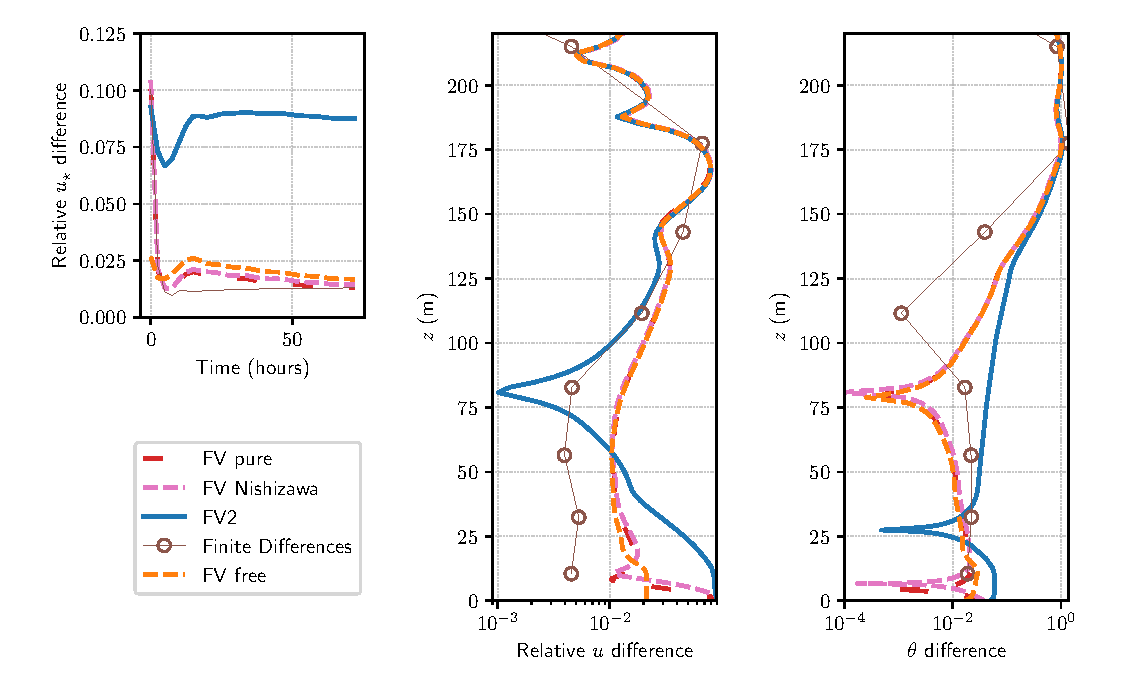
\includegraphics[scale=0.6]{images/consistency_comparisonStratified.pdf}
	\caption{Differences in $u_\star, ||u||$ and $\arg(u)$
	between a high resolution and a low resolution
	of the surface flux schemes presented in a stable
	stratification.
	}
	\label{fig:ND_Consistency_comparisonStratified}
\end{figure}
\paragraph{Results} The differences between the two simulations are shown in Figure
\ref{fig:ND_Consistency_comparisonStratified}.
The difference between the high resolution and the low resolution
does not significantly change with the surface flux schemes.
The difference in $u_\star$ is especially high for the ``FV2" scheme.
Note that the initialization for FV free and FV2 is particular:
to ensure the continuity of the solution,
the initial profile is already adjusted for the
MO theory. This is why the relative $u_\star$ difference is zero
at initialization whereas it is very high for the other surface flux
schemes.
%
The ``FV2" scheme is not very consistent because it follows the
continuous model with $\delta_{\rm a}$ changing together with the
space step.
The Finite Difference or the ``FV pure" methods suffer
less from this problem because even if $\delta_{\rm a}$ changes,
it is assumed that the evolution equation is
integrated inside the surface layer.
\citep{maronga_improved_2020} also find that the
sensitivity of their LES model to the grid spacing is
``\textit{more
likely related to under-resolved near-surface gradients
and turbulent mixing at the boundary-layer top, to the
[sub-grid scale] model formulation, and/or to numerical issues,
and not to deficiencies due to the use of improper surface
boundary conditions}".
\subsection{Study of the consistency: unstable case}
\begin{figure}
	\centering
	\includegraphics[scale=0.6]{images/consistency_comparisonUnstable.pdf}
	\caption{Differences (bottom) in $u_\star, t_\star, ||u||$ and $\theta$
	between a high resolution and a low resolution
	of the surface flux schemes presented in an unstable
	stratification. The corresponding profiles
	with the low resolution simulations are shown in
	the top panels.
	}
	\label{fig:ND_Consistency_comparisonUnstable}
\end{figure}
Figure \ref{fig:ND_Consistency_comparisonUnstable}
shows the differences found between a high resolution simulation
and a low resolution simulation in an unstable situation.
\paragraph{Description of the test case}
To design a test case with an unstable stratification
the sea surface temperature is forced to follow a daily oscillation
between $279$ K and $281$ K.
The initial profiles of temperature and wind
are set to constant values of respectively $280$ K and
$8 \; {\rm m}.{\rm s}^{-1}$.
As in the stable case the geostrophic wind is
$u_G = 8 \;{\rm m}.{\rm s}^{-1}$
and the time step is $\Delta t = 30 \;{\rm s}$.
The ``low resolution" is composed of 50 grid levels of $10 \; m$
each; 15 additional stretched levels between $500 \; m$ and
$1080 \; m$ make sure that the upper boundary condition
is not involved in the results.
The ``high resolution" divides every space levels into
3 space levels of equal size.
\paragraph{Results}
Figure \ref{fig:ND_Consistency_comparisonUnstable}
shows that the ``FV2" scheme is also less consistent
in the unstable case.
This time in the first $200$ meters the scheme ``FV free" seems a lot
more robust than the other schemes.
However, above this height the differences between the high
resolution and the low resolution simulations oscillate and there
is no clear conclusion that can be made.
As in the stable case, the schemes that assume an evolution equation
inside the surface layer are not very sensitive to the choice of
the height of the surface layer.
The main conclusion is hence that
\textbf{if Monin-Obukhov profiles are enforced in the
surface layer the importance of the choice of
$\delta_{\rm a}$ increases.}
In both cases, the different profiles are very similar.
A ocean-atmosphere coupled case is presented in Section
\ref{sec:ND_Consistency_Coupled}, where the surface scheme may be of a greater
importance.
\subsection{Study of the consistency: coupled case}
\label{sec:ND_Consistency_Coupled}
\begin{figure}
	\centering
	\subimport{images/}{algo_schwarz_ND_OA.pdf_tex}
	\caption{Schwarz algorithm applied to ocean-atmosphere
		coupling}
	\label{fig:ND_Consistency_schwarz_algo}
\end{figure}
\begin{figure}
	\centering
	\includegraphics[scale=0.6]{images/consistency_comparisonCoupled.pdf}
	\caption{Same as Figure
	\ref{fig:ND_Consistency_comparisonUnstable} but the sea
	surface temperature $\theta_s$ and surface currents
	$u(0)$ are obtained with a coupled ocean column model.}
	\label{fig:ND_Consistency_comparisonCoupled}
\end{figure}
We now introduce an oceanic column model below the
atmospheric model.
Figure \ref{fig:ND_Consistency_comparisonCoupled}
shows the differences found between a high resolution simulation
and a low resolution simulation in an unstable situation of
this coupled system.
\paragraph{Description of the test case}
In this test case everything is identical to the
unstable case except for the sea surface temperature
$\theta_s$ and the surface current $u(0)$.
Instead of prescribing these values directly,
a Schwarz algorithm is used: the first iteration
begins with the atmosphere and corresponds to
the unstable test case.
The atmosphere is integrated in time
and sends its turbulent fluxes $u_\star^2$ and
$u_\star \theta_\star$ to the ocean model, which
returns the surface values $u(0)$, $\theta_s$.
This process is iterated (see Figure
\ref{fig:ND_Consistency_schwarz_algo}) and
Figure \ref{fig:ND_Consistency_comparisonCoupled} shows
the state of the atmospheric model after 3 iterations.
\par
The ocean model will be described in Chapter
\ref{ch:OceanND} (Finite Differences, $\delta_o=0$).
It is forced with radiative fluxes
to model a diurnal cycle:
\begin{itemize}
\item
	a shortwave (positive downward) heat flux
	\begin{equation}
		Q_{sw}=\max(0,Q_{\max} \cos(2\pi d))
	\end{equation}
	penetrates in the first few levels of the ocean ($d$ is
	the time in days and $Q_{\max} = 500 {\rm W}.{\rm m}^{-2}$);
\item  a longwave (positive downward) heat flux
	$Q_{lw} = -\frac{Q_{\max}}{\pi}$ is applied at the surface.
	Its value corresponds to the daily-averaged $Q_{sw}$.
\end{itemize}
\paragraph{Results}
Figure \ref{fig:ND_Consistency_comparisonCoupled}
shows in its top panels $u_\star$, $\theta_\star$ and
the vertical profiles of $||u||$, $\theta$ in the atmosphere
after 3 Schwarz iterations with the ocean model.
First, note that the oscillations of $u_\star$ and $\theta_\star$
are of a smaller amplitude than in the unstable experiment.
Then, in the bottom panel, one can see that the difference
in $u_\star$ and $u$ between high and low resolutions when using
the ``FV free" scheme is smaller than with the other schemes.
Unlike the previous cases, the ``FV2"
scheme do not show a lot of differences between
its high and low resolutions.
Finally, the dependency of $t_\star$ and $\theta$ on the resolution
was attenuated by the coupling with the ocean column.
\section{Partial conclusion}
In fluid dynamics, having a rough surface requires to exclude from
the computational domain a surface layer. A vast majority of models
use Monin-Obukhov Similarity Theory (MOST)
to avoid solving the small scales of motion inside the surface layer.
We compared several strategies for the treatment of the surface layer
and proposed one (``FV free") with two main assets:
\begin{itemize}
	\item one can choose freely the height $\delta_{\rm a}$
		of the surface layer;
	\item MOST is enforced in the surface layer which avoids
		a contradiction between the evolution equation and
		MOST (that is quasi-stationary).
\end{itemize}
We compared the strategies by verifying that a high-resolution
discretisation would be close to the low-resolution one.
The strategy ``FV free" shows less differences between
high- and low-resolution simulations than the other strategies,
especially for the wind speed and in unstable situations.
\par
In the comparison, we used a Finite Volume method based on spline
reconstruction. This method encourages us to be
clean in the derivation of the discretisation: using the wall law
for the surface viscosity together with the quadratic spline
reconstruction in the surface layer led to an unphysical behaviour.
On the other hand, this method also allows to choose the
reconstruction to follow the wall law.
